% !TEX encoding = UTF-8 Unicode 
% !TEX root = praca.tex

\chapter{Projekt filtrów cyfrowych}

\section{Akwizycja danych eksperymentalnych}

W celu zaprojektowania filtrów zbadano na początku nieprzetworzony sygnał otrzymany prosto
od makiety sprzętowej. W jej oprogramowaniu wyłączono wszystkie funkcje wstępnego przetwarzania
sygnału na czas doświadczenia.
Do odbierania i zapisu sygnału do pliku użyto aplikacji na komputer osobisty wspomnianej w pracy.
W trakcie akwizycji elektrody były podpięte do skóry na ciele autora pracy, w konfiguracji
omówionej w rozdziale 1. Całe doświadczenie trwało około 1 minuty i 18 sekund. Autor pozostawał
w pozycji siedzącej, w bezruchu. Sygnał próbkowano z częstotliwością $f_s = 360Hz$. 
Całość zapisanego sygnału oraz jego fragment w funkcji czasu przedstawiono na wykresach na rysunkach
\ref{fig:sigall} i \ref{fig:sigpart}.

\begin{figure}[h!]
    \centering 
    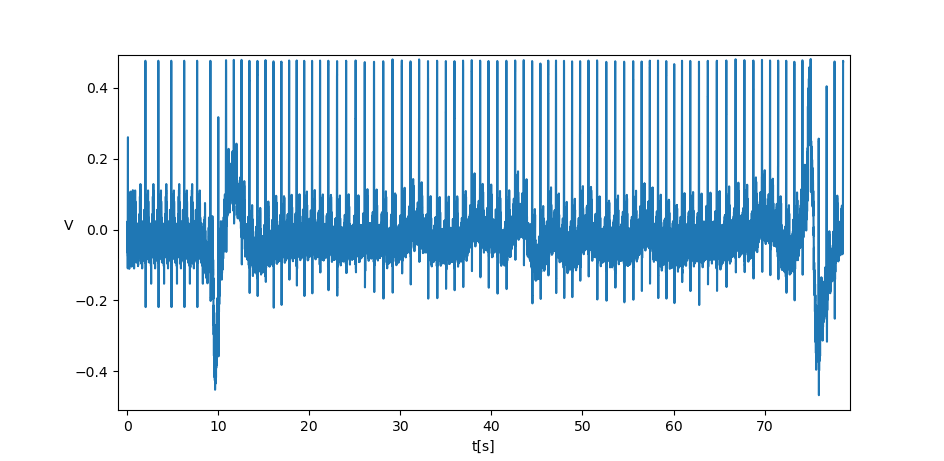
\includegraphics[scale=0.45]{pl/media/sigall.png}
    \caption{Wykres całości odebranego sygnału w funkcji czasu}
    \label{fig:sigall}
\end{figure}

\begin{figure}[h!]
    \centering 
    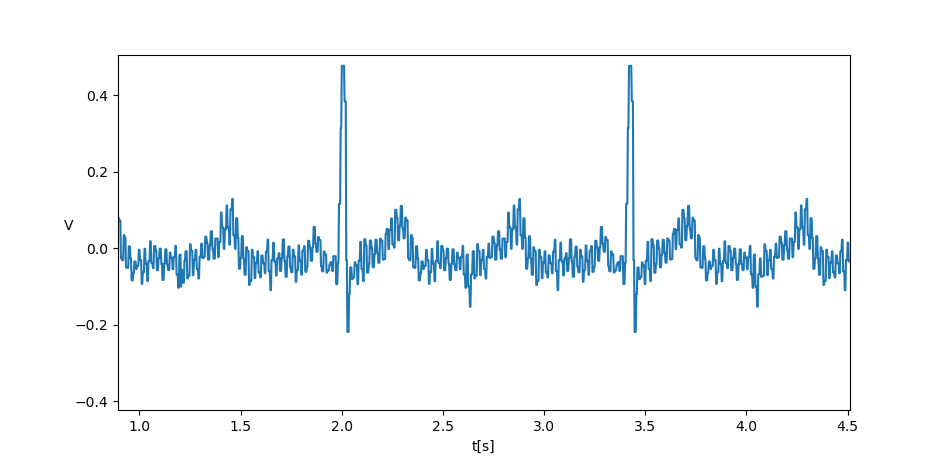
\includegraphics[scale=0.45]{pl/media/sig_unfiltered.png}
    \caption{Wykres fragmentu nieprzetworzonego sygnału w funkcji czasu}
    \label{fig:sigpart}
\end{figure}

\newpage

\section{Analiza sygnału}

Poza analizą wzrokową sygnału na wykresach w dziedzinie czasowej, użyto również dyskretnej 
transformacji Fouriera (a dokładniej implementacji szybkiej transformacji Fouriera - \textit{FFT};
\textit{Fast Fourier Transform}) do analizy sygnału w dziedzinie częstotliwościowej. 
Na listingu \ref{listing:fft} przedstawiono fragment skryptu w języku
\textit{Python}, w którym zastosowano implementację \textit{FFT} dostarczoną przez bibliotekę
\textit{SciPy}. Skrypt z poniższego listingu wczytuje sygnał z pliku tekstowego zapisanego
przez aplikację i wykonuje szybką transformację Fouriera poprzez wykonanie funkcji
\textit{fft}, która zwraca wartości funkcji sygnału po transformacji. 

Na samym końcu zastosowano bibliotekę \textit{matplotlib} do wygenerowania wykresu
połowy wykresu (o nieujemnych wartościach argumentów) sygnału w dziedzinie częstotliwości.

\begin{listing}
\begin{minted}{python}
from scipy.fft import fft, fftfreq
import numpy as np
import matplotlib.pyplot as plt 
import sys 

if len(sys.argv) != 2:
    print("Usage: fft.py <path to the signal file *.txt>")
    sys.exit(1)

y = []
# załadowanie sygnału z pliku tekstowego
with open(sys.argv[1]) as file:
    for line in file:
        y.append(float(line))            

# wykonanie transformacji Fouriera
T = 1.0 / 360.0
N = len(y)
x = np.linspace(0.0, N*T, N, endpoint=False)
yf = fft(y)
xf = fftfreq(N, T)[:N//2]

# wyświetlenie wykresu
plt.plot(xf, 2.0/N * np.abs(yf[0:N//2]))
plt.grid()
plt.show()
\end{minted}
    \caption{Skrypt wykonujący transformację Fouriera i generujący wykres 
sygnału w dziedzinie częstotliwości}
\label{listing:fft}
\end{listing}

\newpage

Na wykresie z rysunku \ref{fig:fftraw} przedstawiono wynik działania skrypty z listingu \ref{listing:fft}. Poniższy
wykres przedstawia sygnał w dziedzinie częstotliwości. Na podstawie tego wykresu możliwe jest określenie 
składowych częstotliwości wpływających na sygnał i ich potencjalne wyeliminowanie poprzez odpowiednio zaprojektowany filtr.
W przedstawionym zakresie spektrum można zaobserwować wyróżniające się spośród reszty składowe częstotliwości, wśród nich m.in.:
$39$, $105$, $112$ i $175 Hz$ oraz częstotliwości poniżej $1 Hz$.

\begin{figure}[h!]
    \centering 
    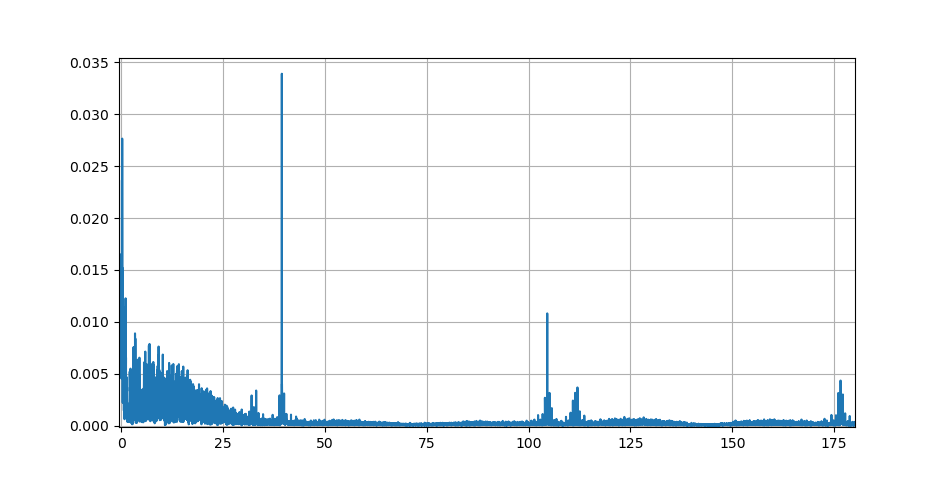
\includegraphics[scale=0.6]{pl/media/fft_raw.png}
    \caption{Fragment wykresu sygnału w dziedzinie częstotliwości}
    \label{fig:fftraw}
\end{figure}

\begin{figure}[h!]
    \centering 
    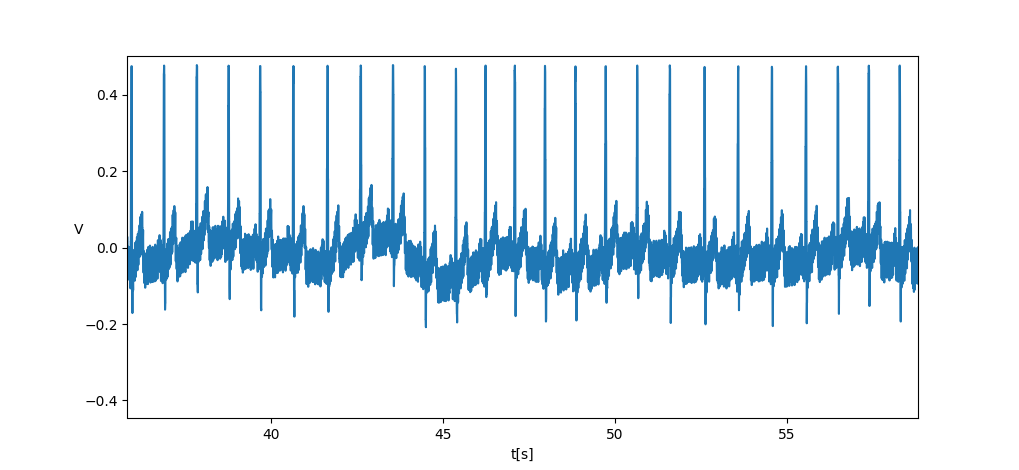
\includegraphics[scale=0.6]{pl/media/baseline_wander.png}
    \caption{Fragment wykresu sygnału w funkcji czasu ilustrujący dryft linii izoelektrycznej}
    \label{fig:baselinewander}
\end{figure}

\newpage

\begin{figure}[h!]
    \centering 
    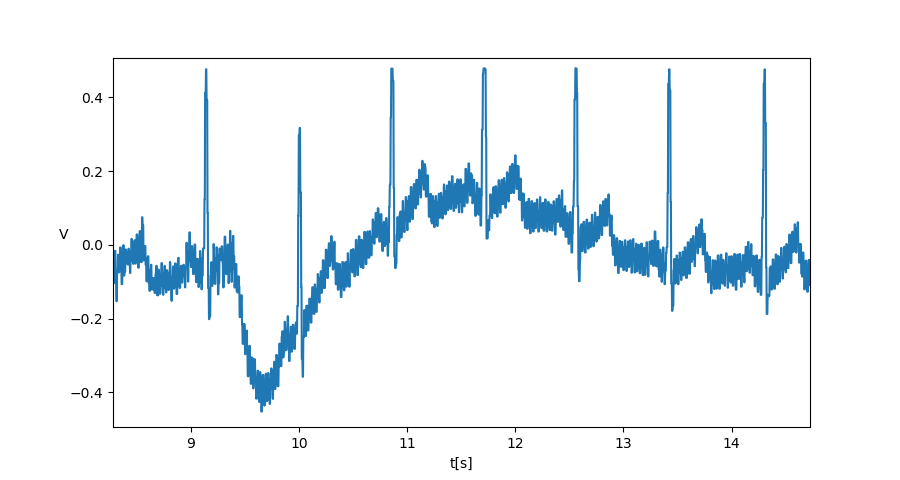
\includegraphics[scale=0.6]{pl/media/wander_2.png}
    \caption{Fragment wykresu sygnału w funkcji czasu szczególnie dotknięty problemem dryftu linii izoelektrycznej}
    \label{fig:wander2}
\end{figure}

Na wykresach z rysunków \ref{fig:baselinewander} i \ref{fig:wander2} przedstawiono dryft linii izoelektrycznej 
na przykładzie analizowanego sygnału, jest to szum o niskiej częstotliwości (zazwyczaj maksymalnie $1-5 Hz$), 
najczęściej powodowany oddechem pacjenta oraz skurczami innych mięśni niż mięśnia sercowego. 
Problem ten sprawia że przejrzysta wizualizacja sygnału (jak również diagnostyka chorób) 
jest utrudniona. 

Na wykresach z rysunków \ref{fig:sigpart} oraz \ref{fig:hfnoise} można zaobserwować szumy o wyższych 
częstotliwościach niż we wzorcowym sygnale EKG (rys. \ref{fig:pqrst}). 
Tego typu szum może utrudnić lub uniemożliwić poprawne rozpoznanie przez wykwalifikowany personel medyczny 
załamków w zespole \textit{PQRST}.

\begin{figure}[h!]
    \centering 
    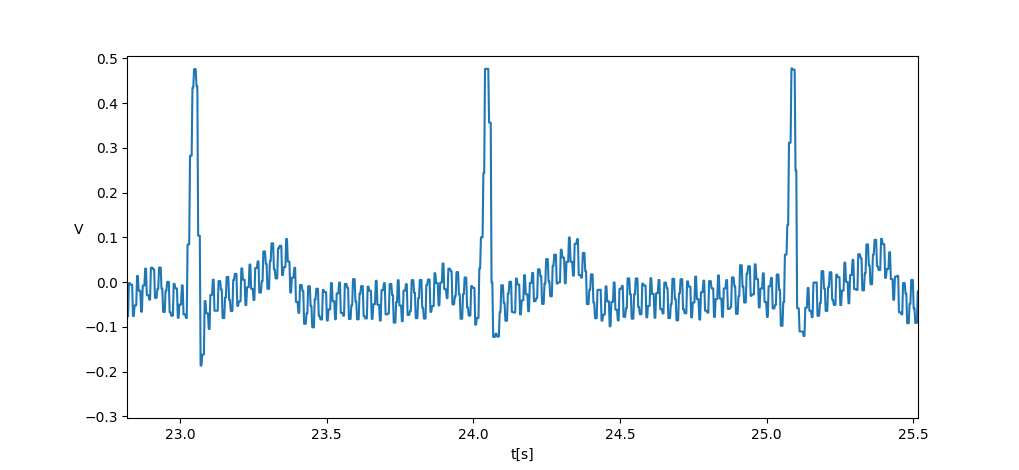
\includegraphics[scale=0.6]{pl/media/high_frequency_noise.png}
    \caption{Fragment wykresu sygnału w funkcji czasu ilustrujący występowanie szumów wysokiej częstotliwości}
    \label{fig:hfnoise}
\end{figure}

\newpage 

\section{Projekt filtrów FIR}

W projektowaniu filtrów o skończonej odpowiedzi impulsowej (\textit{FIR}) posłużono się skryptem napisanym w języku \textit{Python}.
Skrypt na podstawie pliku konfiguracyjnego w formacie \textit{YAML} \cite{yaml}, oblicza współczynniki filtrów FIR z zadanymi parametrami. 
Przykładowy plik konfiguracyjny podano na listingu \ref{listing:yaml}.

\begin{listing}
\begin{minted}{yaml}
default:
  f_sampling: 360
  window: "blackman"
  ntaps: 63 

fir0:
  f_cutoff: 30 
  pass_zero: True 

fir1:
  f_cutoff: 8 
  pass_zero: False 
\end{minted}
    \caption{Pliku konfiguracyjny dla skryptu obliczającego współczynniki filtrów}
\label{listing:yaml}
\end{listing}
 
Na powyższym listingu wartości pod \textit{default:} 
są parametrami domyślnymi projektowanych filtrów. Następnie
widoczne są definicje parametrów dla dwóch filtrów o nazwach roboczych \textit{fir0} i 
\textit{fir1}. Możliwe jest ustawienie wartości następujących parametrów:

- \textit{f\_sampling} - określa częstotliwość próbkowania w $Hz$,

- \textit{window} - łańcuch znaków będący nazwą funkcji okna stosowanej w projekcie filtru,

- \textit{ntaps} - liczba wyjściowych współczynników filtru,

- \textit{f\_cutoff} - częstotliwość odcięcia w $Hz$,

- \textit{pass\_zero} - wartość prawda/fałsz (\textit{True}/\textit{False}), w przypadku
prawdy projektowany filtr jest filtrem dolnoprzepustowym, w przeciwnym razie górnoprzepustowym.
Dla każdego z filtrów \textit{fir0} i \textit{fir1} skrypt stworzy pliki wynikowe \textit{fir1.txt}
oraz \textit{fir1.txt} z listą współczynników w formacie tekstowym.

Na listingu \ref{listing:pyfir} przedstawiono fragment wspomnianego skryptu. Do wczytywania
i interpretacji zawartości pliku \textit{YAML}, wykorzystano bibliotekę \textit{PyYAML} \cite{PyYAML}.
Natomiast do zaprojektowania filtru użyto funkcji \textit{firwin} z biblioteki \textit{SciPy}.
Funkcja ta zwraca listę z wartościami wyliczonych współczynników filtru na podstawie zadanych
parametrów.

\begin{listing}
\begin{minted}{python}
from scipy.signal import firwin
import yaml, sys

if len(sys.argv) != 2:
    print("Usage: fir_design.py <.yml file path>")    
    sys.exit(1)

with open(sys.argv[1], "r") as file:
    yml = yaml.load(file, Loader=yaml.Loader)

for filter_name in yml:
    if filter_name == "default":
        continue
    params = yml["default"]

    for param in yml[filter_name]:
        params[param] = yml[filter_name][param]

    coeffs = firwin(
            fs =        params["f_sampling"], 
            cutoff =    params["f_cutoff"], 
            numtaps =   params["ntaps"], 
            pass_zero = params["pass_zero"], 
            window=     params["window"]
        )
# (...)
\end{minted}
    \caption{Fragment skryptu wspomagającego projektowanie filtrów FIR}
\label{listing:pyfir}
\end{listing}

\begin{listing}
\begin{minted}{python}
from scipy import signal
import numpy as np
import matplotlib.pyplot as plt
import sys
# (...)
y = []

with open(sys.argv[1]) as file:
    for line in file:
        y.append(float(line))        

w, h = signal.freqz(y, fs=360)
# (...)
\end{minted}
    \caption{Fragment skryptu generującego wykres charakterystyki częstotliwościowej filtrów}
\label{listing:freqz}
\end{listing}


Poza skryptem wspomagającym zaprojektowanie filtru, stworzono również skrypt (listing
\ref{listing:freqz}) generujący wykres charakterystyki częstotliwościowej danego filtru. 
W skrypcie tym zastosowano standardowe funkcje do wyświetlania wykresu z biblioteki \textit{matplotlib} oraz funkcję \textit{freqz} z biblioteki \textit{SciPy}. 

\newpage

\begin{figure}[h!]
    \centering 
    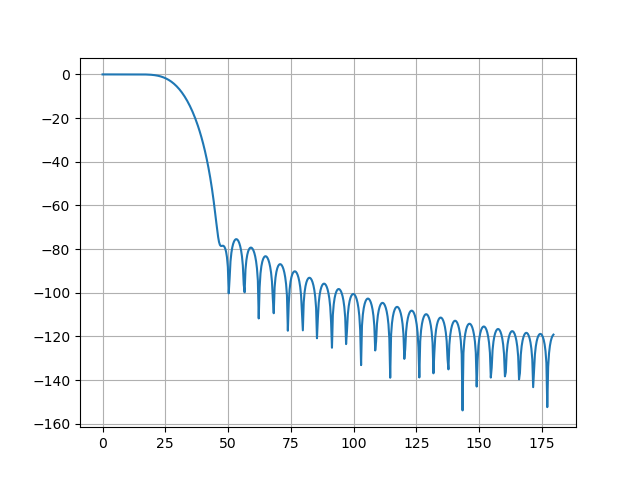
\includegraphics[scale=0.5]{pl/media/lpf.png}
    \caption{Wykres charakterystyki częstotliwościowej filtru dolnoprzepustowego} 
    \label{fig:lpf}
\end{figure}

\begin{figure}[h!]
    \centering 
    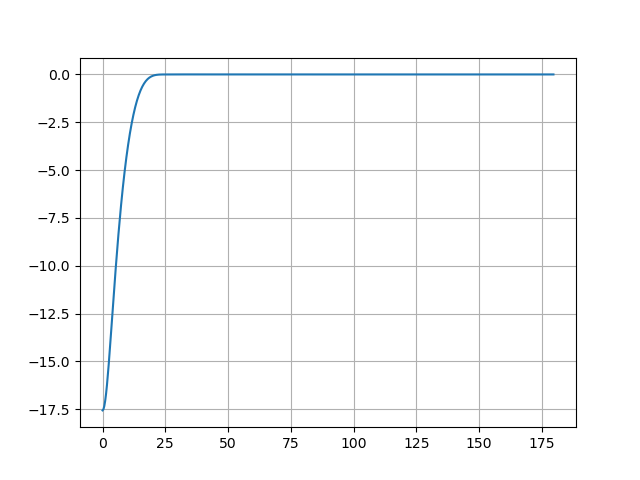
\includegraphics[scale=0.5]{pl/media/hpf.png}
    \caption{Wykres charakterystyki częstotliwościowej filtru górnoprzepustowego} 
    \label{fig:hpf}
\end{figure}

Na wykresach z rysunków
\ref{fig:lpf} i \ref{fig:hpf} przedstawiono charakterystyki częstotliwościowe filtrów
o parametrach zawartych w pliku z listingu \ref{listing:yaml}. Zaprojektowane
w ten sposób filtry zastosowano w pracy, umieszczając współczynniki w pamięci mikrokontrolera.
Korzystając z implementacji splotu dyskretnego w oprogramowaniu sprzętowym zrealizowano
filtrację sygnału w czasie rzeczywistym.

Na wykresie z rysunku \ref{fig:hpsig} przedstawiono sygnał po zastosowaniu samego
filtru górnoprzepustowego. Zauważyć można, że dzięki zastosowaniu filtru górnoprzepustowego,
dla większości fragmentów sygnału w znaczący sposób zredukowano wpływ dryftu linii izoelektrycznej.
Natomiast na wykresie z rysunku \ref{fig:lpsig} przedstawiono fragment wykresu sygnału
po zastosowaniu filtru \textit{fir0}. Dzięki zastosowaniu tego filtru, po pozbyciu
się części szumów wysokiej częstotliwości można wyraźniej zaobserwować załamki \textit{PQRST}. 
Na rysunku \ref{fig:filtfft} przedstawiono wykres po filtracji sygnału 
przedstawiony w dziedzinie częstotliwościowej. Zaobserwowano, że wcześniej występujące
nieregularności w paśmie powyżej $25 Hz$ zostały zredukowane, jak również w paśmie
poniżej $5 Hz$.

\begin{figure}[h!]
    \centering 
    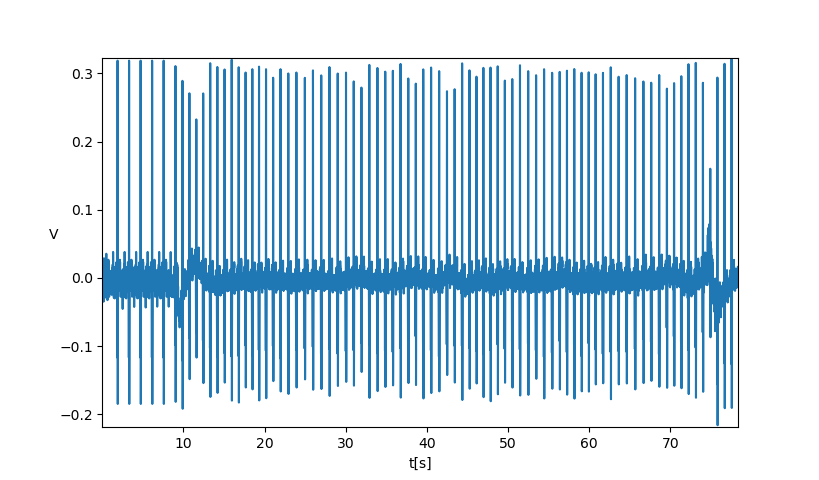
\includegraphics[scale=0.5]{pl/media/hpsig.png}
    \caption{Wykres sygnału w czasie po zastosowaniu filtru górnoprzepustowego (\textit{fir1})} 
    \label{fig:hpsig}
\end{figure}

\begin{figure}[h!]
    \centering 
    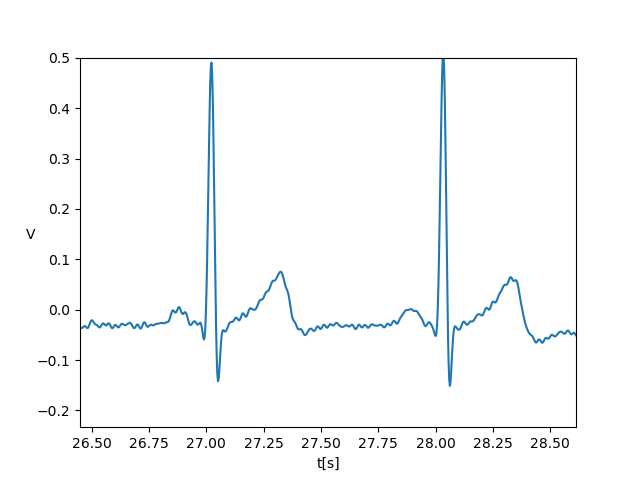
\includegraphics[scale=0.5]{pl/media/lpsig.png}
    \caption{Fragment wykresu sygnału w czasie po zastosowaniu 
    filtru dolnoprzepustowego (\textit{fir0})} 
    \label{fig:lpsig}
\end{figure}


\begin{figure}[h!]
    \centering 
    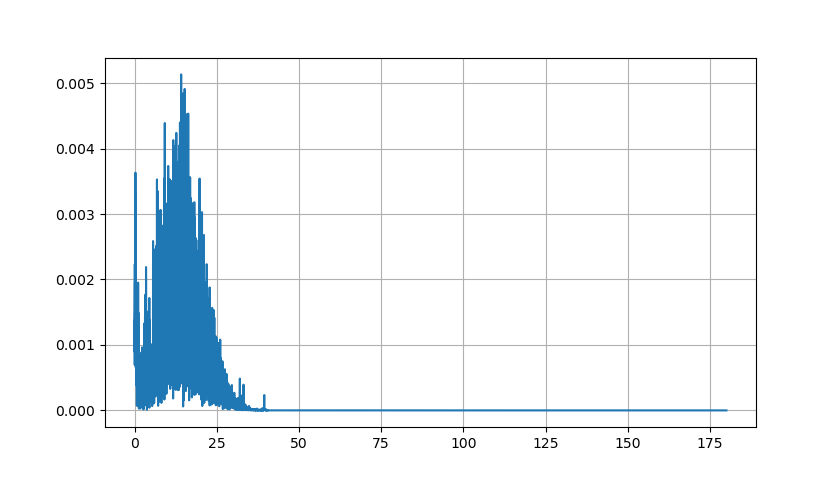
\includegraphics[scale=0.5]{pl/media/fftall.png}
    \caption{Wykres sygnału po zastosowaniu fitrów \textit{fir0} oraz \textit{fir1} 
    i transformacji Fouriera} 
    \label{fig:filtfft}
\end{figure}

